% figures/trace_example.tex
% Example optionized proof trace with solver annotations

\begin{figure}[t]
\centering
\footnotesize
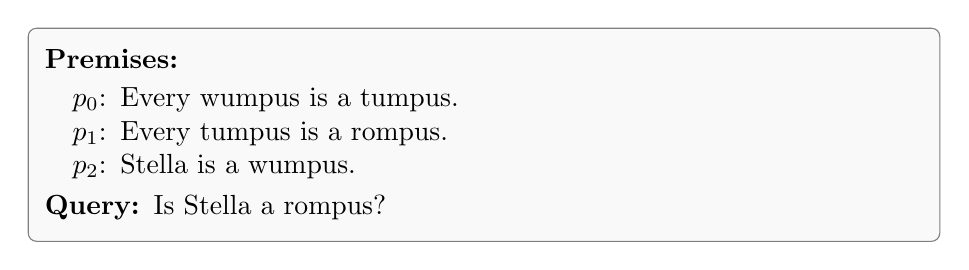
\begin{tikzpicture}
\node[draw=black!50, rounded corners=3pt, fill=gray!5, inner sep=6pt, text width=0.92\columnwidth] {
\begin{tabular}{@{}l@{}}
\textbf{Premises:}\\[2pt]
\hspace{1em}$p_0$: Every wumpus is a tumpus.\\
\hspace{1em}$p_1$: Every tumpus is a rompus.\\
\hspace{1em}$p_2$: Stella is a wumpus.\\[3pt]
\textbf{Query:} Is Stella a rompus?\\
\end{tabular}
};
\end{tikzpicture}

\vspace{0.4em}
\rule{0.92\columnwidth}{0.4pt}
\vspace{0.3em}

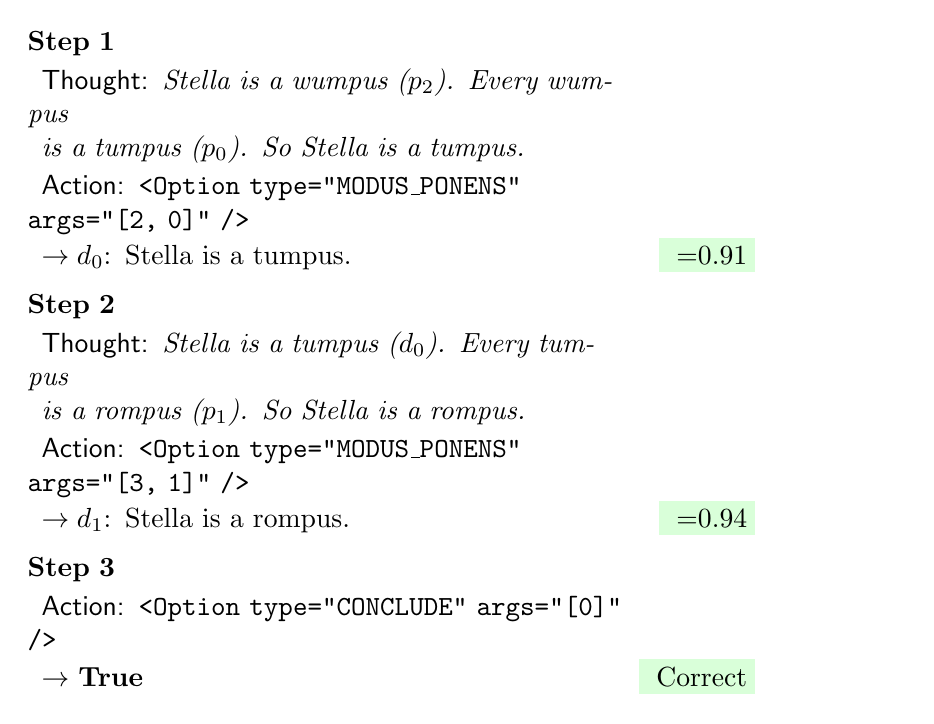
\begin{tikzpicture}
\node[text width=0.92\columnwidth, inner sep=0pt] {
\begin{tabular}{@{}p{0.68\columnwidth}@{\hspace{0.5em}}r@{}}
\textbf{Step 1} & \\[2pt]
\hspace{0.5em}\textsf{Thought:} \textit{Stella is a wumpus ($p_2$). Every wumpus} & \\
\hspace{0.5em}\textit{is a tumpus ($p_0$). So Stella is a tumpus.} & \\[2pt]
\hspace{0.5em}\textsf{Action:} \texttt{<Option type="MODUS\_PONENS" args="[2, 0]" />} & \\[2pt]
\hspace{0.5em}$\rightarrow d_0$: Stella is a tumpus. & \colorbox{green!15}{{\color{green!50!black}\checkmark} $\qhat{=}0.91$} \\[6pt]

\textbf{Step 2} & \\[2pt]
\hspace{0.5em}\textsf{Thought:} \textit{Stella is a tumpus ($d_0$). Every tumpus} & \\
\hspace{0.5em}\textit{is a rompus ($p_1$). So Stella is a rompus.} & \\[2pt]
\hspace{0.5em}\textsf{Action:} \texttt{<Option type="MODUS\_PONENS" args="[3, 1]" />} & \\[2pt]
\hspace{0.5em}$\rightarrow d_1$: Stella is a rompus. & \colorbox{green!15}{{\color{green!50!black}\checkmark} $\qhat{=}0.94$} \\[6pt]

\textbf{Step 3} & \\[2pt]
\hspace{0.5em}\textsf{Action:} \texttt{<Option type="CONCLUDE" args="[0]" />} & \\[2pt]
\hspace{0.5em}$\rightarrow$ \textbf{\textsc{True}} & \colorbox{green!15}{{\color{green!50!black}\checkmark} Correct} \\
\end{tabular}
};
\end{tikzpicture}
\caption{Example optionized proof trace. Each step includes a natural language \textsf{Thought}, a structured \textsf{Action} (option with arguments), the derived formula, and solver validity with $\qhat$ prediction.}
\label{fig:trace_example}
\end{figure}
